
\begin{appendix}

\section{Sch\'ema de discr\'etisation spatiale VEF}
\label{section-VEF}

Le sch\'ema VEF de TrioCFD est d\'ecrit succinctement dans ce qui suit, afin de pouvoir pr\'eciser les axes de progr\`es possibles et
justifier les voies futures propos\'ees dans la section \ref{Progres-VEF}.\\

Pour introduire le sch\'ema VEF, on consid\'ere un probl\`eme mod\`ele simplifi\'e par rapport au probl\`eme r\'eellement r\'esolu dans le code.
Il d\'ecrit l'\'ecoulement stationnaire d'un fluide incompressible isotherme soumis \`a un champ de forces quelconque.

\subsection{Probl\`eme mod\`ele continu}
 
 Soit le probl\`eme \`a r\'esoudre, en dimension $d$ de l'espace ($d=2$ ou $d=3$): 

\begin{equation}
\label{NS_isoT_stat}
\left\lbrace
\begin{array}{lcll}
%
\ds{- \nu \Delta  \mathbf{u} + \left( \mathbf{u}\cdot \nabla \right) \mbf{u}+\nabla P }
&=&
\ds{ \mathbf{f},}
&\ds{ \mbf{x}\in \Omega\subset \mathbb R^d,}\\
\\
\ds{\nabla\cdot\mathbf{u}}
&=&
0,
&\ds{ \mbf{x}\in \Omega},\\
\\
\ds{ \mbf{u}}
&=&
\mbf{0},
&\ds{ \mbf{x}\in  \partial \Omega}.
\end{array}
\right.
\end{equation}


Soient $X=\mbf{H}^1_0(\Omega )^d$ et $Q=L_0^2 (\Omega )$. 
La formulation faible du probl\`eme continu (\ref{NS_isoT_stat}) est : \\

\begin{equation}
\label{Stokes_form_continu}
\left\lvert
\begin{array}{l}
\ds{ \text{Trouver } (\mbf{u},p)\in X\times Q  \text{ tels que } \forall (\mbf{v},q)\in X\times Q }\\
\\
\ds{a(\mbf{u}, \mbf{v})+c(\mbf{u}, \mbf{u}, \mbf{v}) + b( \mbf{v}, \mbf{p})=l(\mbf{v}) }\\
\\
\ds{b(\mbf{u},\mbf{q}) =0.}
\end{array}
\right.
\end{equation}

Ici, $ a: X\times X \longrightarrow \mathbb R $ et $ b: X\times Q \longrightarrow \mathbb R $ sont deux formes bilin\'eaires continues,
$ c: X\times X \times X\longrightarrow \mathbb R $ est une forme trilin\'eaire continue et $ l: X \longrightarrow \mathbb R $
une forme lin\'eaire continue. Ces formes sont donn\'ees par:

\begin{equation}
\ds{
a(\mbf{u}, \mbf{v}):= \nu \int _{\Omega}\nabla \mbf{u}: \nabla \mbf{v}\ dx
}
\end{equation}

\begin{equation}
\ds{
b (\mbf{u},{q}) =-\int _{\Omega} q \nabla \cdot \mbf{u}\ dx
}
\end{equation}

\begin{equation}
\ds{
c \left(  \mbf{a}, \mbf{u}, \mbf{v} \right) = \int _{\Omega}
  \left(  \left( \mbf{a}\cdot \nabla \right) \mbf{u} \right) \cdot \mbf{v}
  \ dx
}
\end{equation}

\begin{equation}
\ds{
l \left(   \mbf{v} \right) =\int _{\Omega}
  f  \mbf{v}
  \ dx
}
\end{equation}

Avant d'introduire le probl\`eme discr\'etis\'e en espace, on introduit quelques notations.

\subsection{Notations}


Soit un maillage $ \ds{\mathcal T _h=\left\lbrace T_m \right\rbrace _{1\leq m\leq N}}$ du domaine de calcul $ \Omega $ en
triangles ou t\'etra\`edres. Pour des domaines \`a fronti\`eres courbes (typiquement les assemblages avec des crayons combustibles)
le maillage $ \mathcal T _h $ ne recouvre pas n\'ecessairement $ \Omega $ \footnote{Ce point pose un probl\`eme de pr\'ecision de la solution
num\'erique en proche paroi.}. On d\'esigne donc par $\Omega _h$ l'int\'erieur de l'ensemble $\ds{ \bigcup _{m=1}^{N}T_m}$.
L'ensemble des faces int\`erieures du maillage est not\'e $\mathcal F _h^i$. On note $ \left\lbrace s_{i,T} \right\rbrace _{i=1}^{d+1}$ les sommets
de l'\'el\'ement $T$. La face oppos\'ee au sommet $s_{i,T}$ est la face $ F_{i,T}$. 


\begin{figure}[h]
\begin{center}
\begin{tabular}{c}
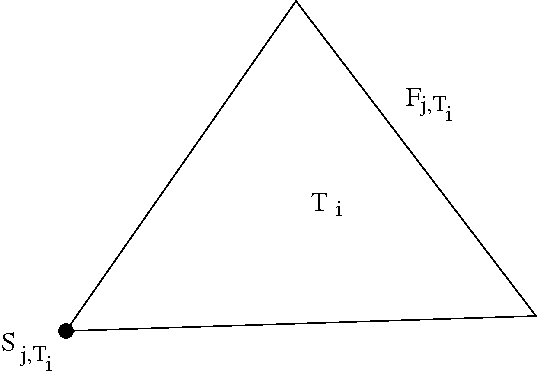
\includegraphics[scale=0.3]{Figs/notations-VEF.png}
\end{tabular}
\end{center}
\caption{Schéma GD sur grille décalée: notations.}
\end{figure}



\subsection{Probl\`eme discr\'etis\'e}
Le sch\'ema peut \^etre exprim\'e comme un sch\'ema VEF ou un sch\'ema de type El\'ements Finis (EF). Les deux approchent diff\`erent essentiellement du point
de vue de l'assemblage de la matrice du syst\`eme \`a inverser et de certains termes (matrice de rigidit\'e et termes sources par exemple) qui ne remettent pas
en cause les id\'ees ici pr\'esent\'ees\footnote{L'\'equivalence entre les formulations VEF et EF est abord\'ee dans \cite{Emonot} et \cite{Heib}.}.
Le formalisme EF permet d'\'etablir certaines preuves de stabilit\'e et de convergence et est choisi ici.\\
Introduisons maintenant le probl\`eme discret.

L'espace d'\'el\'ements finis de Crouzeix-Raviart est d\'efini comme suit :

\begin{equation}
\label{Xh}
\ds{
X_h = \left\lbrace \mbf{v}_h \in \mbf{L}^2(\Omega_h); \forall T \in \mathcal T _h, \mbf{v}_{h}\vert T\in \mathbb P^1(T); \forall F \in \mathcal F _h^i, \int _F  \llbracket \mbf{v}_h \rrbracket _F =0 \right\rbrace
}
\end{equation}
 
 o\`u $ \llbracket . \rrbracket _F $ d\'esigne le saut sur la face $F$.

La vitesse discr\`ete  est d\'efinie par

\begin{equation}
\label{vh_faces}
\ds{
\mbf{v}_h(\mbf{x}) = \sum _{F\in \mathcal F_h}\sigma _F(\mbf{v}_h)\mathbb I _F(\mbf{x}),\ \mbf{x}\in \Omega _h.
}
\end{equation}

avec

\begin{equation}
\ds{
\sigma _F(\mbf{v}_h) \equiv \frac{1}{mes(F)}\int _F \mathbf {v}_h\  ds=\mbf{v}_h(\mbf x _F).
}
\end{equation}

\begin{rque}
Puisque le saut de $ \mbf{v}_h $ est lin\'eaire sur $F$, la condition $\int _F  \llbracket \mbf{v}_h \rrbracket =0$ est \'equivalente \`a la continuit\'e de $ \mbf{v}_h $ au barycentre de $F$.
\end{rque}

 Si $\mbf v _h \in X_h$ alors sur chaque \'el\'ement $T$ on peut \'ecrire

\begin{equation}
\ds{
  \mbf{v}_{h\vert T} =\sum _{i=1}^{d+1} \sigma_{T,i}\theta _{T,i} \in \mathbb P^1(T),\ \sigma_{T,i}= \mbf{v}_{h\vert T} (\mbf{m}_i).
}
\end{equation}

où $ \ds{\theta _{T,i} = 1-d\lambda_{T,i}}$  avec  $\lambda _i$ la coordonn\'ee barycentrique associ\'ee au sommet  $i$ de $ T$ : $ \ds{\lambda _{T,i} = 1 }$ au sommet $s_{i,T}$ et $0$ aux autres sommets. 




Dans (\ref{vh_faces}), la fonction $\varphi _F$ appartient \`a l'espace $X_h $ et son support est constitu\'e du ou des deux simplexes contenant $F$. Sur ces deux simplexes,
elle co\"\i ncide
avec la fonction de forme de l'\'el\'ement fini de Crouzeix-Raviart associ\'ee \`a $F$ \`a savoir : si la face $F$ correspond \`a la face $F_i$ de l'\'el\'ement $T$ alors $\varphi _{F\vert T} = \theta _{T,i}$.\\
Ainsi, on peut exprimer la vitesse discr\`ete en se ramenant \`a une sommation sur les \'el\'ements du maillage :

\begin{equation}
\label{vh_elts}
\ds{
\mbf{v}_h(\mbf{x}) = \sum _{T\in \mathcal F_h} \left( \sum _{i=1}^{d+1} \sigma_{T,i} \theta _{T,i} \right) \mathds{1} _T, \mbf{x}\in \Omega _h,
}
\end{equation}






Il existe diff\'erentes variantes du sch\'ema VEF, qui diff\`erent les unes des autres dans le calcul de la pression discr\`ete. Dans la version de base du sch\'ema VEF, on approche le champ
de pression par le calcul d'une valeur moyenne de la solution sur chaque \'el\'ement. Il s'agit de la th\`ese de P. Emonot \cite{Emonot}. Cet espace a ensuite \'et\'e enrichi dans les
th\`eses de S. Heib \cite{Heib} et de T. Fortin \cite{Fortin} pour am\'eliorer la stabilit\'e du sch\'ema et obtenir des propri\'et\'es de super-convergence.\\

Soit 

\begin{equation}
\ds{
Q_h^0 = \left\lbrace q_h\in L_0^2(\Omega _h): q_{h|T} \in \mathbb P^0(T)\ \forall T\in \mathcal T _h\right\rbrace.
}
\end{equation}

Une fonction $q_h^0\in Q_h^0$ s'\'ecrit 

\begin{equation}
\ds{
q_h^0(\mbf x)=\sum _{T\in \mathcal T h}q_T\Psi _T(\mbf x) },
\end{equation}

 avec $\Psi _T(\mbf x)=1 $ si $\mbf x\in T$, $0$ sinon. Le degr\'e de libert\'e $q_T$ associ\'e au triangle $T$ s'interpr\`ete comme une approximation de la moyenne de la solution sur
 l'\'el\'ement:

\begin{equation}
\ds{q_T=\frac{1}{mes(T)}\int _T q(\mbf x)\ d\mbf x.}
\end{equation}

Un autre espace d'approximation pour la pression a ensuite \'et\'e introduit par S. Heib \cite{Heib}, pour r\'eduire l'apparition de certains modes parasites en vitesse. Il introduit des
degr\'es de libert\'e en pression aux sommets des \'el\'ements :

\begin{equation}
\ds{
Q_h^1 = \left\lbrace q_h\in \mathcal C ^0(\Omega _h): q_{h|T} \in \mathbb P^1(T) \ \forall T\in \mathcal T _h\right\rbrace
}
\end{equation}

Une fonction $q_h^1\in Q_h^1$ s'\'ecrit 

\begin{equation}
\ds{q_h^1(\mbf x)=\sum _{T\in \mathcal T h}\left( \sum _{i=1}^{d+1} q_h(\mbf s _i)\varphi _i (\mbf x)\right) \mathbb 1 _T(\mbf x) } 
\end{equation}

Enfin, T. Fortin \cite{Fortin} a propos\'e d'ajouter des degr\'es de libert\'e en pression sur chaque ar\^ete des \'el\'ements :


\begin{equation}
\ds{
Q_h^a = \left\lbrace q_h\in \mathcal C ^0(\Omega): q_{h|T} \in \mathbb P_T^a\ \forall T\in \mathcal T _h\right\rbrace,
}
\end{equation}


Une fonction $q_h^a\in Q_h^a$ s'\'ecrit 

\begin{equation}
\ds{q_h^a(\mbf x)=\sum _{T\in \mathcal T h}\ \sum _{a=1}^{d+1} q_h(a_T)\mathbb I _a (\mbf x) }.
\end{equation}




Le probl\'eme discret s'\'ecrit : 

\begin{equation}
\left\lvert
\label{pb-VEF-P0}
\begin{array}{l}
\ds{ \text{Trouver } (\mbf{u}_h,p_h)\in X_h\times Q_h  \text{ tels que}\ \forall (\mbf{v}_h,q_h)\in X\times Q_h }\\
\\
\ds{a_h(\mbf{u}_h, \mbf{v}_h)+c_h(\mbf{u}_h, \mbf{u}_h, \mbf{v}_h) + b_h( \mbf{v}_h, \mbf{p}_h)=l_h(\mbf{v}_h) }\\
\\
\ds{b_h(\mbf{u_h},\mbf{q_h}) =0.}
\end{array}
\right.
\end{equation}



avec

\begin{equation}
\left\lbrace
\begin{array}{l}
\ds{
a_h(\mbf{u}_h, \mbf{v}_h):= \nu \sum _{\mathcal T _h}\int _{T}\nabla \mbf{u}_h: \nabla \mbf{v}_h\ dx
}\\
\\
\ds{
c_h \left(  \mbf{u}_h, \mbf{u}_h, \mbf{v}_h \right) = \sum _{\mathcal T _h}\int _{T}
  \left(  \left( \mbf{u}_h\cdot \nabla \right) \mbf{u}_h \right) \cdot \mbf{v}_h
  \ d\mbf x.}
\end{array}
\right.
\end{equation}

La d\'efinition de la forme bilin\'eaire $b_h$ d\'epend de l'espace d'approximation retenu pour la pression.\\

$ \bullet $ {\bf{ Schéma $\mathbb P^1$ NC / $\mathbb P^0 $ :}} $q_h=q_h^0\in Q_h^0.$\\

\begin{equation}
\ds{
b_h (\mbf{u}_h,q_h)=-\sum _{T\in \mathcal T _h}\nabla \mbf{u}_h q_h^0\ d\mbf x.
}
\end{equation}

$ \bullet $ {\bf{ Schéma $\mathbb P^1$ NC / $\mathbb P^0 \mathbb P^1$ :}} $q_h=q_h^0 + q_h^1\in Q_h^0 + Q_h^1$ \\

\begin{equation}
\ds{
b_h (\mbf{u}_h,q_h)=\sum _{T\in \mathcal T _h}\int _T \left( \mbf{u}_h\nabla  q_h^1- q_h^0 \nabla \mbf{u}_h \right) \ d\mbf x. 
}
\end{equation}

$ \bullet $ {\bf{ Sch\'ema $\mathbb P^1$ NC / $\mathbb P^0 \mathbb P^1 \mathbb P^a$ (3D uniquement)}} : $q_h=q_h^0 + q_h^1 + q_h^a \in Q_h^0 + Q_h^1 + Q_h^a$.\\

\begin{equation}
\ds{
b_h (\mbf{u}_h,q_h)=\sum _{T\in \mathcal T _h}\int _T \left( \mbf{u}_h\nabla  \left(q_h^1 + q_h^a \right) - q_h^0 \nabla \mbf{u}_h \right) \ d\mbf x.  
}
\end{equation}




\begin{figure}[h]
\begin{center}
\begin{tabular}{cc}
\hline \rowcolor{lightgray}
El\'ement de Crouzeix-Raviart & El\'ement $\mathbb P^1$ NC / $\mathbb P^0 \mathbb P^1$ \\
\hline
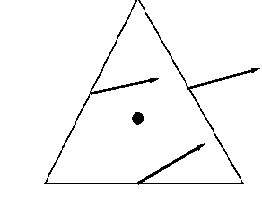
\includegraphics[scale=0.5]{Figs/VEF-P0.png}&
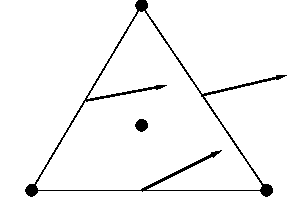
\includegraphics[scale=0.5]{Figs/VEF-P0P1.png}
\end{tabular}
\end{center}
\caption{Degr\`es de libert\'e du sch\'ema VEF en 2D en vitesse (fl\^eches) et pression (ronds).}
\end{figure}

\begin{figure}[h]
\begin{center}
\begin{tabular}{ccc}
\hline \rowcolor{lightgray}
El\'ement de Crouzeix-Raviart & El\'ement $\mathbb P^1$ NC / $\mathbb P^0 \mathbb P^1$  &El\'ement $\mathbb P^0 \mathbb P^1 \mathbb P^a$\\
\hline
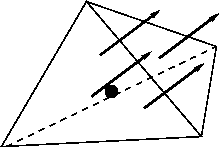
\includegraphics[scale=0.5]{Figs/VEF-3D-P0.png}&
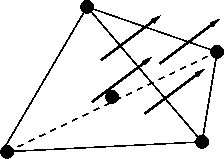
\includegraphics[scale=0.5]{Figs/VEF-3D-P0P1.png}&
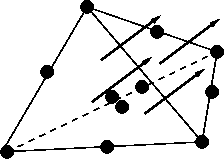
\includegraphics[scale=0.5]{Figs/VEF-3D-P0P1Pa.png}
\end{tabular}
\end{center}
\caption{Degrés de liberté du schéma VEF en 3D en vitesse (flèches) et pression (ronds).}
\end{figure}


En pratique, la m\'ethode $\mathbb P^0 \mathbb P^1 \mathbb P^a$, qui n\'ecessite le calcul de $11$ degr\'es de libert\'e en pression par \'el\'ement n'est pas utilis\'ee car trop
co\^uteuse, malgr\`e les propri\'et\'es de stabilit\'e et de convergence d\'emontr\'ees dans \cite{Fortin}. L'\'el\'ement de Crouzeix-Raviart, stable uniquement pour le probl\`eme de
Stokes, n'est pas utilis\'e. Seule la variante  $\mathbb P^0 \mathbb P^1$ est en g\'en\'eral consid\'er\'ee. 

\subsection{Termes de convection non-linéaires}
\label{section-annexe-convection}

Diff\'erents sch\'emas num\'eriques sont impl\'ement\'es pour la discr\'etisation du terme de convection.  On d\'ecrit ici les plus utilis\'es, \`a savoir:

\begin{itemize}
\item
les sch\'emas d\'ecentr\'es  {\sc{amont}} et {\sc{muscl}}, de type volumes finis,
\item
le sch\'ema centr\'e {\sc{EF}} et le sch\'ema d\'ecentr\'e {\sc{EF\_stab}}.
\end{itemize}

Ces sch\'emas diff\`erent les uns des autres par la m\'ethode de d\'ecentrement utilis\'ee, qui se traduit par une dissipation num\'erique plus ou moins importante.

Afin de simplifier la pr\'esentation, nous nous restreignons au cas bi-dimensionnel.
Nous rappelons que dans la formulation VEF \`a chaque degr\'e de libert\'e $x_i$ de la vitesse, on associe un volume de contr\^ole $w_i$ (voir~Fig.$\ref{vdc}$). 

Nous avons:

$$\int_{w_i} \div (\velocity \otimes \velocity) dV =  \int_{\gamma_i} \velocity (\velocity . \normal ) ds,  $$
o\`u $\gamma_i$ d\'esigne les faces du volume de contr\^ole $w_i$.


\begin{figure}[h!]
\centering
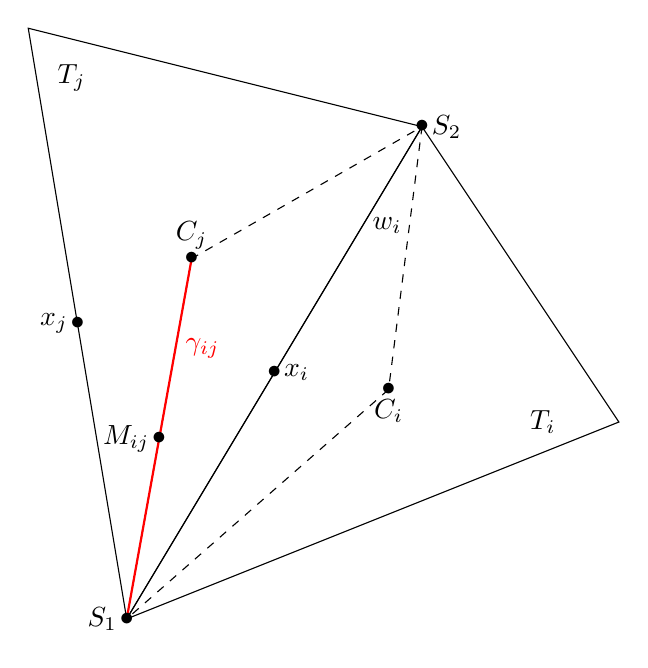
\begin{tikzpicture}[scale=1.25]%,cap=round,>=latex]

\coordinate  (S1) at (3cm,0cm);
\coordinate  (S2) at (6cm,5cm);
\coordinate  (A) at (2cm,6cm);
\coordinate  (B) at (8cm,2cm);
\coordinate  (Cj) at (3.66cm,3.66cm);
\coordinate  (Ci) at (5.66cm,2.33cm);
\coordinate  (xj) at (2.5cm,3cm);
\coordinate  (xi) at (4.5cm,2.5cm);
\coordinate  (M) at (3.33cm,1.83cm);

\draw (S1) -- (S2) -- (A) --  (S1);
\draw (S1) -- (S2) -- (B) --  (S1);
\draw [dashed] (S1) -- (Cj) -- (S2) --  (Ci) -- (S1);

\draw [thick, red] (Cj) -- (S1) node[near start, right] {$\gamma_{ij}$};

\draw (Ci) node[below] {$C_i$};
\draw (Cj) node[above] {$C_j$};
\draw (Ci) node {$\bullet$};
\draw (Cj) node {$\bullet$};

\draw (xi) node[right] {$x_i$};
\draw (xj) node[left] {$x_j$};
\draw (xi) node {$\bullet$};
\draw (xj) node {$\bullet$};

\draw (S1) node[left] {$S_1$};
\draw (S2) node[right] {$S_2$};
\draw (S1) node {$\bullet$};
\draw (S2) node {$\bullet$};

\draw (M) node[left] {$M_{ij}$};
\draw (M) node {$\bullet$};

\draw (7,2) node[right] {$T_i$};
\draw (2.2,5.5) node[right] {$T_j$};
\draw (5.4,4) node[right] {$w_i$};



\end{tikzpicture}
\caption{Volume de contr\^ole}
\label{vdc}
\end{figure}

{\bf{Sch\'ema  {\sc{amont}}}}\\

Dans le sch\'ema d\'ecentr\'e amont $\velocity_i$ est approch\'e, par exemple sur $\gamma_{ij} = w_i  \cap w_j$, par $\velocity_i$ si $(\velocity . \normal_{ij} ) > 0 $, et par $\velocity_j$ si $(\velocity . \normal_{ij} <0)$, o\`u  $\normal_{ij}$ repr\'esente la normale unitaire ext\'erieure \`a $\gamma_{ij}$:

$$\int_{\gamma_{ij}} \velocity (\velocity . \normal ) ds \approx \int_{\gamma_{ij}} \velocity_i \max(\velocity . \normal_{ij}, 0) + \velocity_j \min(\velocity . \normal_{ij}, 0). $$ 


{\bf{Sch\'ema  {\sc{muscl}}}}\\



Dans le sch\'ema {\sc{muscl}}  (Monotone Upstream-Centred Scheme for Convective flows), le flux \`a travers la face $\gamma_{ij}$ est approch\'e \`a partir de la formule d'interpolation de Simpson:


$$\int_{\gamma_{ij}} \velocity (\velocity . \normal ) ds \approx \frac{ \mid  \gamma_{ij} \mid}{6}  \left( \velocity_{S_1} \vect{U}_{S_1}  + 4 \velocity_{M_{ij}} \vect{U}_{M_{ij}} +   \velocity_{C_j} \vect{U}_{C_j} \right), $$

o\`u nous avons utilis\'e les notations repr\'esent\'ees dans Fig. $\ref{vdc}$ et, si $\velocity_{M_{ij}} .  \normal_{ij} > 0$ :

%\begin{equation*}
 % \left\{
\begin{align*}
\vect{U}_{S_1} &=  \velocity_{i} + \mid x_j S_1 \mid  \nabla(\velocity_i) ,\\
\vect{U}_{M_{ij}} &=  \velocity_{i} + \mid x_j M_{ij} \mid \nabla(\velocity_{i}) , \\
\vect{U}_{C_j} &= 2 \velocity_{M_{ij}} - \velocity_{S_1} ,\\
\end{align*}
%\right.
%\end{equation*} 

sinon, 

%\begin{equation*}
%  \left\{
\begin{align*}
\vect{U}_{S_1} &=  \velocity_{j} + \mid x_j S_1 \mid \nabla(\velocity_j) ,\\
\vect{U}_{M_{ij}} &=  \velocity_{j} + \mid x_j M_{ij} \mid \nabla(\velocity_{j}) , \\
\vect{U}_{C_j} &= 2 \velocity_{M_{ij}} - 2\velocity_{S_1}.
\end{align*}
%\right.
%\end{equation*}  



Diff\'erents limiteurs de pente sont utilis\'es afin de calculer le $\nabla(\velocity_{i})$ \`a partir des gradients associ\'es aux triangles $T_i$ et $T_j$ partageant la face $S_1S_2$:


$$ \nabla (\velocity_{i})  =
 \begin{cases}
   \text{minmod}(\nabla(\velocity_{T_i}); \nabla(\velocity_{T_j})) ,\\
 \text{Van-Leer} (\nabla(\velocity_{T_i}); \nabla(\velocity_{T_j})) , \\
\text{Van-Albanda}(\nabla(\velocity_{T_i}); \nabla(\velocity_{T_j})) , 
\end{cases}
$$


La fonction $\text{minmod}$ est d\'efinie par 

\begin{equation*}
\text{minmod} (a,b)=\begin{cases}0, & \text{si } a \cdot b \leq 0, \\ 
a, & \text{si } \mid a \mid <   \mid b \mid , \quad a \cdot b > 0,\\
b, &  \text{si } \mid a \mid >  \mid b \mid , \quad a \cdot b > 0, \end{cases}
\end{equation*} 

la fonction $\text{Van-Leer} $ est d\'efinie par

\begin{equation*}
\text{Van-Leer} (a,b)=\begin{cases}0, & \text{si } a \cdot b \leq 0, \\ 
\dfrac{2 a \cdot b}{ a + b}, & \text{sinon },\\
 \end{cases}
\end{equation*} 

et $\text{Van-Albanda}$ par

\begin{equation*}
\text{Van-Albanda} (a,b)=\begin{cases}0, & \text{si } a \cdot b \leq 0, \\ 
\dfrac{ a \cdot b \cdot (a+b)}{ a^2 + b^2}, & \text{sinon }.\\
 \end{cases}
\end{equation*} 




%
%\section{Point sur le projet TrioCFD}
%
%%\begin{turn}{90}
%%{\rowcolors[\hline]{3}{almond}{pastelgray}
%\begin{tabular}{|l|l|l|l|l|}
%\hline\rowcolor{almond} \bf \phantom & \bf Avant    & \bf Apr\`es   & \bf Objectifs & \bf \'etat d'avancement  fin 2018\\
%\rowcolor{almond}  & \bf   restructuration & \bf  restructuration & \bf \phantom & \bf    \\
%\hline
%\cellcolor{almond} \bf{HPC}  & de pointe & en retard & R\&D \`a reprendre & D\'emarr\'ee (Lot 8)\\
%\cellcolor{almond} \bf et performances &  &  & &+ actions {\sc{Trust} } \\
%\cellcolor{almond} \bf  &  &  & &  (GT HPC) \\
%
%\hline\cellcolor{almond}\bf{Architecture  }&  innovante &  p\'erenne & \`a consolider& actions {\sc{Trust}}\\
%\cellcolor{almond}\bf{ informatique }&                  &                & (augmentation & \\
%\cellcolor{almond}\bf{  }&                  &                & du nombre & \\
%\cellcolor{almond}\bf{  }&                  &                & d\rq{}applications) & \\
%\hline
%\cellcolor{almond}\bf{Gros maillages}& avanc\'e & en retard & R\&D \`a reprendre& pr\'evu Lot 8\\
%\cellcolor{almond}&  &  &  (r\'esolution de gros syst\`emes& + actions {\sc{Trust}}\\
%\cellcolor{almond}&  &  &   lin\'eaires mal conditionn'es)&  \\
%\hline
%\cellcolor{almond}\bf{Num\'erique}& sch\'ema original &  sch\'ema original  & \`a am\'eliorer  & Actions engag\'ees  \\
%\cellcolor{almond}& et performant &et performant   &et diversifier  &   (Lot 1, Lot 4, Lot 5) \\
%\cellcolor{almond}\bf{}&  &   & (maillages quelconques,  & \\
%\cellcolor{almond}\bf{}&  &   & ordre \'elev\'e,...) & \\
%\hline
%\cellcolor{almond}\bf{Mod\'elisation }& LES en phase & retard  & \`a consolider &  Nouveau mod\`ele: \\
%\cellcolor{almond}\bf{ (turbulence)}&  avec R\&D ouverte &   &  &  $(k,\epsilon)$ r\'ealisable \\
%\cellcolor{almond} &   &   &  &    + actions Lot 3\\
%\hline
%\cellcolor{almond}\bf{Mod\'elisation }&\'el\'ementaire  &\'el\'ementaire  & \`a remplacer &  Action engag\'ee (Lot 7)\\
%\cellcolor{almond}\bf{(porosit\'e) }&   &  & par m\'ethode   &  \\
%\cellcolor{almond}\bf{ }&   &  &plus pr\'ecise  &  \\
%\cellcolor{almond}\bf{ }&   &  &(\rq\rq{}CFD poreuse\rq\rq{}) &  \\
%\hline
%\cellcolor{almond}\bf{R\&D}& tr\`es active &  arr\^et & red\'emarrage &  3 th\`eses en cours  \\
%\cellcolor{almond}&  &   &  &  1 post-doc \\
%\cellcolor{almond}&  &   &  &    GT interne LMSF, \\
%\cellcolor{almond}&  &   &  &    projet ANR CINE-PARA\\
%\hline
%\cellcolor{almond}\bf{ Fonctionnalit\'es  }&chimie simplifi\'ee  & & & Mod\`ele compressible \\
%\cellcolor{almond}\bf {originales  }& rayonnement & pertes&Nouvelles  &  (Lot 9.1, pr\'evu en 2019)\\
%\cellcolor{almond}\bf {  }& suivi particules & comp\'etences&fonctionnalit\'es  & Particules solides \\
%\cellcolor{almond}\bf {  }&...  & &  &   polydisperse \\
%\cellcolor{almond}\bf {  }& & &  &   (Lot 9.2, pr\'evu en 2019)\\
%\cellcolor{almond}\bf {  }&  & &  &   IFS  (Lot 2, en cours)\\
%\hline
%\cellcolor{almond}\bf { Positionnement}&\'etudes r\'ealis\'ees   &  arr\^et&{\bf{Exploitation en production~:}}  & \\
%\cellcolor{almond}\bf {de l'outil au CEA}&par le CEA \`a la   & &Agr\'e\'e OCS pour  ASTRID  & actions  prospectives\\
%\cellcolor{almond}\bf { et chez les}&demande des   & & mise en OpenSource & en cours:\\
%\cellcolor{almond}\bf {partenaires}&partenaires & &  {\bf{Nouvelles niches~:}}  & \\
%\cellcolor{almond}\bf {  }&(pas de mise    & &  IFS(coeurs et GV)& d\'eveloppement ALE \\
%\cellcolor{almond}\bf {  }&  en production)  & &  assemblages combustibles&m\'ethode multi-\'echelles \\
%\hline
%\cellcolor{almond}\bf{Convivialit\'e }& mauvaise & am\'elior\'ee & IHM  & Pr\'evu en 2019\\
%\cellcolor{almond}\bf{de l'outil }& & &   & \\
%\hline
%\end{tabular}
%%}
%%\end{turn}



\section{D\'ecouplage des op\'erateurs transport et chimie}
\label{section-decouplage}

 Le syst\`eme de transport r\'eactif peut s'\'ecrire, dans le cas d'un milieu poreux non-d\'eformable satur\'e:

$$
\left\{
\begin{array}{lcl}
\partial _t \omega \vec{c}  & = &  \displaystyle
 \underbrace{\vec{{\cal L}}}_{\color{blue}transport} + \underbrace{{S}^T}_{\color{blue} stoe.} ~ \vec{r}  \\
\omega  & = & \displaystyle \omega ^0
\frac{1+f_{mv}^0}{1+f_{mv}} \mbox{ avec } f_{mv} = \sum _j {\cal V}_j^{mol} f_j  \\
 \Phi _{\chi}(\omega,\vec{c},\vec{r}) & = & 0 \\
\end{array}
\right.
$$

\bigskip

$\omega $ repr\'esente la porosit\'e et $f_{mv}$ la fraction volumique r\'eactive de la phase solide. Attention: les concentrations des esp\`eces chimiques solides 
sont ici calcul\'ees en fonction du volume de la phase liquide et non solide. Cela peut para\^itre contre-intuitif mais c'est un point de vue fr\'equemment adopt\'e, 
dans le cadre de la chimie des transferts entre phase liquide et solide. 

\bigskip

Nous savons par le th\'eor\`eme du rang que, si les \'equations chimiques sont toutes ind\'ependantes (i.e. si le probl\`eme chimique est bien pos\{), alors il existe une matrice $U$ telle que $US^T = $ matrice nulle.  Donc en posant $\vec{u} = U\omega \vec{c}$, nous avons $\partial _t \vec{u} = U \partial _t \omega \vec{c} = U\vec{\cal L}
+ U{S}^T ~ \vec{r} = U\vec{\cal L}$  

$\vec{u}$ est souvent appel\'e vecteur des {\color{blue} composants}, c'est-\`a-dire des invariants chimiques, obtenu par combinaison lin\'eaire des concentrations des esp\`eces. 

\begin{enumerate}
\item Nous r\'esolvons alors le syst\`eme de transport {\color{blue}lin\'eaire et global} suivant:
$$
\partial _t \vec{u} =   U\vec{\cal L}  
$$
\item Nous utilisons la valeur calcul\'ee de $\vec{u}$ pour en d\'eduire $\vec{c}$ par un ensemble de syst\`emes chimiques {\color{blue} non-lin\'eaires et locaux}:
$$
\left\{
\begin{array}{lcl}
U\omega \vec{c}  & = &  \displaystyle
  \vec{u}  \\
\Phi _{\chi}(\omega,\vec{c},\vec{r}) & = & 0 \\
\omega  & = & \displaystyle \omega ^0
\frac{1+f_{mv}^0}{1+f_{mv}} \\
\end{array}
\right.
$$


\end{enumerate}

On peut proc\'eder de mani\`ere s\'equentielle ou it\'erative entre les \'etapes 1 et 2. 


\end{appendix}
